\documentclass[tikz]{standalone}
\usetikzlibrary{decorations.shapes,decorations.markings,decorations.pathreplacing}

\tikzset{
    set arrow inside/.code={\pgfqkeys{/tikz/arrow inside}{#1}},
    set arrow inside={end/.initial=>, opt/.initial=},
    /pgf/decoration/Mark/.style={
        mark/.expanded=at position #1 with
        {
            \noexpand\arrow[\pgfkeysvalueof{/tikz/arrow inside/opt}]{\pgfkeysvalueof{/tikz/arrow inside/end}}
        }
    },
    arrow inside/.style 2 args={
        set arrow inside={#1},
        postaction={
            decorate,decoration={
                markings,Mark/.list={#2}
            }
        }
    },
}
\begin{document}
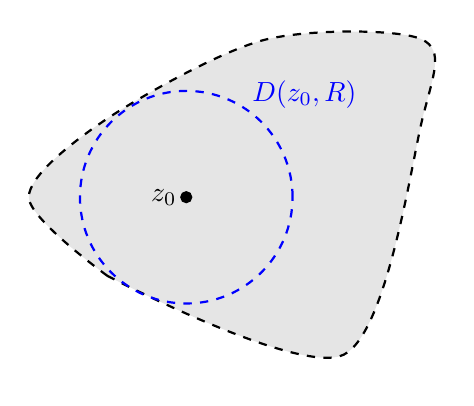
\begin{tikzpicture}
\draw[thick,dashed,fill=gray!20] plot [smooth] coordinates {(0,0) (-1,1) (0,2) (2,3) (4,3) (4,2) (3,-1) (0,0)};
\draw[fill] (1,1) circle(2pt);
\draw (1,1) node[left]{$z_0$};
\draw[blue] (2.5,2.3) node[]{$D(z_0,R)$};
\draw[thick,dashed,blue] (1,1) circle(1.35);
%\draw[fill] (3.5,1.5) circle(2pt);
%\draw (3.5,1.5) node[below]{$z_2$};
%\draw[thick,dashed,red] (3.5,1.5) circle(0.25);
%\draw[red,->] (4.2,1.5) node[right]{$D(z_2,r_2)$} -- (3.8,1.5);
\end{tikzpicture}
\end{document}